\section{Projektumsetzung}
\label{sec:Projektumsetzung}

Aufbauend auf einer konkreten Projekt- und Umsetzungsidee kann die Umsetzung des Projektes begonnen werden.
Die Umsetzung erfasst dabei die Vorbereitung der Projektrealisierung, die eigentliche Realisierung des Projektes
und die Nachbereitung der Realisierung in Form eines Projekttests und einer Anwenderdokumentation. 

\subsection{Projektorganisation}
\label{sec:Projektorganisation}

Die Vorbereitung der Umsetzung des beschriebenen Projektes beginnt mit der Festlegung der Projektorganisation.
Eine Betrachtung der Projektorganisation ist an dieser Stelle von besonderem Interesse, da die Projektorganisation
den Ordnungsrahmen des Projektes festlegt.
Dieser Ordnungsrahmen dient dazu das zielgerichtete Zusammenwirken
der Projektmitglieder und den reibungslosen Projektablauf sicherzustellen.\footnote{\citet[S.~15]{geiger2009}}

Eine besondere Herausforderung an die Projektorganisation des vorliegenden Projektes ergibt sich hierbei
aus dem angesprochenen Projektumfeld (siehe Abschnitt \nameref{sec:Projektumfeld}). Die Projektmitglieder sind
nicht nur mit der Arbeit am Projekt beschäftigt, sondern zeitgleich auch mit Aufgaben im jeweiligen
Unternehmen, mit anstehenden Prüfungsleistungen und mit Arbeitsleistungen in anderern Modulen.
Die Projektorganisation muss diese Teilung der Arbeitskraft berücksichtigen und daher genügend Flexibilität
besitzen und gleichzeitig eine effiziente Aufgabenverteilung gewährleisten. Darüber hinaus muss
die Zerlegung von Aufgaben in Teilaufgaben und die dezentrale Erarbeitung dieser Teilaufgaben unterstützt werden.

Vor diesem Hintergrund wird die Managementmethode Scrum\footnotemark\ zur Umsetzung der Organisation ausgewählt.
Die Scrum-Methode schafft eine einheitliche Organisationsstruktur, 
indem die Aufgaben des Projekts in Arbeitspakete eingeteilt werden,
die in einem festen Zyklus abgearbeitet werden. Zur Verdeutlichung wird die Scrum-Organisation in \abbildung{Scrum}
dargestellt:

\footnotetext{Scrum ist im ursprünglichen Sinn ein Managementframework, mit dem die die Erstellung von Produkten,
durch Verbesserung und Teilung der Arbeitsaufgaben, effzienter gestaltet werden sollen (vgl. \citet[S.~6]{gloger2013})}

\clearpage
\begin{figure}[htb] 
\centering
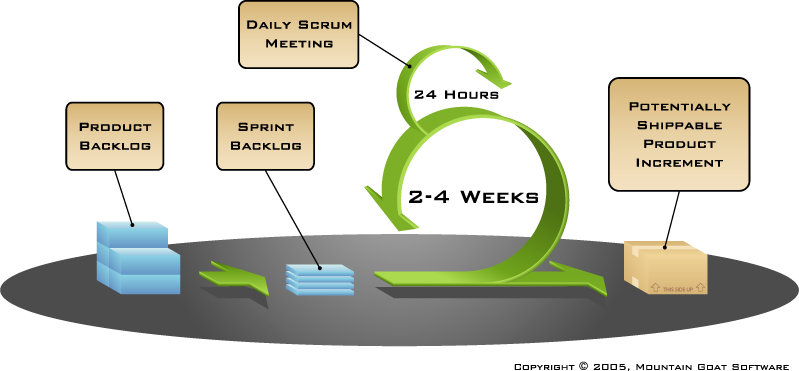
\includegraphics[width=1.0\textwidth]{Scrum.png}
\caption[Scrum-Organisation]{Schematische Organisation eines Projektes mit der Scrum-Methode\protect\footnotemark}
\label{fig:Scrum}
\end{figure}
\footnotetext{Quelle: \url{www.fossa.de}}

Das dargestellte Modell zeigt, dass der Projektinhalt zerteilt und in iterativen Schritten erarbeitet wird. Dieses
Vorgehen schafft, durch die Teilung in zwei iterative Teilprozesse, die nötige Flexibilität der Projektorganisation.
Zum einen ist im Scrum-Modell ein Bearbeitungsprozess vorgesehen
der in zwei bis vier Wochen durchlaufen wird. Dieses Zeitintervall wurde im vorliegenden Projekt für die Erreichung des
nächsten Meilensteins\footnotemark\ vorgesehen. Zum anderen ist ein kleineres Zeitintervall von einem Tag dargestellt, das
genutzt wurde, um kleinere Teilaufgaben auf dem Weg zum nächsten Meilenstein fertig zu stellen.

\footnotetext{Meilensteine stellen elementare Stationen im Verlauf des Projektes dar. Eine genauere Beschreibung
folgt im weiteren Verlauf.}

Durch die Scrum-Organisation konnten kleine Teilaufgaben dezentral bearbeitet werden, ohne die zentrale Erreichung des
nächsten Meilensteins aus den Augen zu verlieren. Eine Projektorganisation, die die aufgezeigten Anforderungen
erfüllt, ist damit definiert.

% \subsubsection*{Möglichkeiten der Projektorganisation}
% \label{sec:MoeglichkeitenProjektorganisation}

% % Scrum ist eine Methode der agilen Softwareentwicklung. Konkret stellt Scrum eine
% % agile Projektmanagementmethode dar. Eine solche Managementmethode behandelt
% % nicht die konkrete Struktur und Art der Zusammenarbeit im Team, sondern
% % beschränkt sich auf den Ablauf des Projektes. Bei einer Projektorganisation nach
% % der Scrum-Methode lassen sich grundsätzlich jeweils drei verschiedene Rollen,
% % Zeremonien und Artefakte unterscheiden. Diese sollen im Folgenden näher
% % beschrieben werden. Die drei zentralen Rollen der Scrum-Methode sind hierbei\ldots

% \subsubsection*{Planung der Projektorganisation}
% \label{sec:PlanungProjektorganisation}

% \subsubsection*{Umsetzung der Projektorganisation}
% \label{sec:UmsetzungProjektorganisation}

% Für eine erfolgreiche Durchführung des Projektes ist es unabdingbar sich vorher
% über die Projektorganisation im Klaren zu sein. Bei der Projektorganisation
% handelt es sich hierbei darum, wie die Entwicklung eines Projektes vonstatten
% gehen soll. Dies bedeutet, dass festgelegt wird, welche Entwicklungsmethodiken
% angewandt werden oder welche Hilfsmittel und Zusatztools eingesetzt werden, um
% das gewünschte Ziel des Projektes möglichst effizient zu erreichen. Ebenfalls
% umfasst dieser Aspekt den Punkt der Kommunikation und Interaktion des
% Projektteams und der einzelnen Projektmitglieder untereinander. Hinzu kommt,
% dass festgelegt wird, wie die einzelnen Meetings der Projektgruppe vonstatten
% gehen und welche Bedingungen erfüllt werden müssen.

% Bei dem großen Umfang und der Vielfalt dieses Projektes ist es notwendig
% flexibel zu sein und somit auf Probleme oder Änderungen und Wünsche des
% Auftraggebers zeitnah reagieren und umsetzen zu können. Um somit die
% Entwicklung agil zu gestalten, entschied man sich in diesem Projekt für die
% Scrum-Methode. Dies ist eine Methodik der agilen Softwareentwicklung und sorgt
% mit sogenannten Scrum-Meetings für regelmäßige Treffen der Projektmitglieder.
% Diese Scrum-Meetings werden immer in gleichen Abständen nach sogenannten
% Sprints gehalten. Die Sprints können hierbei 1 bis 30 Tage lang sein und
% stellen einzelne Iterationsschritte in der Entwicklung der Anwendung dar. Nach
% jeweils einem Sprint, entsteht eine weitere lauffähige Anwendung, aber um die
% Funktionen des letzten Sprints erweitert. Somit wird gewährleistet, dass immer
% eine lauffähige Version zur Verfügung steht und dem Auftraggeber vorgelegt
% werden kann. Nach Ablauf eines Sprints und des darauffolgenden
% Scrum-Meetings,werden weitere Arbeitspakete und Aufgaben an die einzelnen
% Projektmitglieder verteilt, welche in dem folgenden Sprint erledigt werden
% müssen. Durch die kurzen Sprints und häufigen Meetings können so Meinungen,
% Ideen und auch Probleme bei der Umsetzung unter den Projektmitgliedern
% diskutiert und beseitigt werden. Hierbei ist jedes Mitglied gleichberechtigt
% involviert. Trotz dessen können bei der Scrum-Methode folgende drei Rollen
% unterschieden werden:

% \begin{description}
% \item[Der Product Owner] stellt einen Vertreter für den Endkunden dar und
% vertritt somit dessen Wünsche und Bedürfnisse hinsichtlich der Anwendung. Der
% Product Owner trifft somit auch die Entscheidungen bzgl. Kosten und weiterer
% gewünschter Änderungen oder Vorgaben. Die Ergebnisse werden ebenfalls von
% diesem überprüft.
% \item[Der Scrum-Master] dient als Schnittstelle zwischen dem Product Owner und
% dem Scrum-Team und fördert die Zusammenarbeit. Ebenfalls sorgt er dafür, dass
% das Scrum-Team nach den Regeln der Scrum-Methode arbeiten.
% \item[Das Scrum-Team] ist für die Entwicklung und Implementierung der
% gewünschten Anwendung zuständig. Es handelt eigenständig und organisiert somit
% sich und die Vorgehensweise in großem Maße selbst.
% \end{description}

% Ebenfalls zu erwähnen ist, dass ein Product-Backlog ein vom Endkunden
% definierter Katalog ist, welcher die Anforderungen des Kunden , nach Priorität
% und Wichtigkeit sortiert, enthält. Die Anforderungen des Product-Backlog werden
% dabei in ein sogenanntes Sprint-Backlog übertragen, welches bei den Sprints als
% Vorlage für die zu erfüllenden Aufgaben dient. Nach jedem Sprint werden die
% erzielten Ergebnisse, unabhängig von der erreichten Vorgaben, in einem Sprint
% Review dokumentiert und an den Product Owner zur Einsicht übergeben.

% In folgender Abbildung wird der Scrum-Prozess nochmals visuell dargestellt:

% Nach einer kurzen Einführung in die agile Softwareentwicklung kann nun gesagt
% werden, dass das Projektteam in diesem Projekt agil entwickelt hat. Dazu wurde
% eine Sprintdauer von einer Woche angesetzt. Nach dieser Woche fand immer ein
% Scrum-Meeting statt, in der die Erkenntnisse und Ergebnisse der einzelnen
% Projektmitglieder reflektiert wurden. Für die einzelnen Scrum-Meetings sind
% ebenfalls Gesprächsprotokolle erstellt worden, auf die im Nachhinein
% zugegriffen werden kann (siehe Anhang). Bei besonders komplexen Problemen
% während der Entwicklung der Anwendung, wurde auf die Methode des Pair
% Programming zurückgegriffen. Dies bedeutet, dass mehrere Mitglieder
% gleichzeitig und zusammen an einem Rechner an einem Implementierungsproblem
% arbeiten. Dadurch konnten komplexe Probleme schneller und effizienter beseitigt
% werden, da sich die Teammitglieder während des Arbeitens direkt austauschen
% können. Zum Schluss jedes Scrum-Meetings wurden ebenfalls neue Arbeitspakete an
% die Gruppenmitglieder verteilt.

% Die Verwaltung der Arbeitspakete wurde dabei durch ein zusätzliches Tool
% realisiert, welches sich PHProjekt nennt. Dieses Tool ist ein webbasiertes
% Ticketsystem, welches es ermöglicht Arbeitspakete einzelnen Gruppenmitgliedern
% zuzuweisen und deren einzelne Status anzeigen zu lassen. Ebenfalls ist es hier
% möglich Prioritäten und Dauer zu definieren, um die wichtigsten Arbeitspakete
% zu kennzeichnen und eine Frist zur Erledigung zu setzen.

% Um die einzelnen Programmversionen, welche nach den Sprints entstehen, zu
% verwalten, wurde die Versionsverwaltung Github eingesetzt, welche ebenfalls
% webbasiert arbeitet. Hiermit ist es möglich Abspaltungen von einer bestehenden
% Programmversion zu erzeugen und diese zu bearbeiten und nach Abschluss wieder
% der Stammversion hinzuzufügen. So kann gewährleistet werden, dass immer eine
% funktionsfähige Version zur Verfügung steht, da isoliert von der Stammversion
% gearbeitet und entwickelt wird.
\subsection{Projektphasen}
\label{sec:Projektphasen}

Nachdem im vorherigen Abschnitt die Organisation des Projektes erläutert wurde,
wird im Folgenden das Projekt in Phasen gegliedert. Die Phasen dienen 
dazu, das Projekt in einem geordneten Ablauf zu strukturieren und
Arbeitsschritte aufeinander aufbauend zu vergeben. "`Der Aufbau der
Projektphasen ist darauf ausgerichtet, systematisch und aufeinander aufbauend
zu 'lernen', um insgesamt eine optimale Entscheidungsprozedur zu
durchlaufen"'.\footnote{\citet{walter2006}}

Jede Projektphase stellt dabei eine in sich geschlossene Einheit dar, die aus
mehreren Arbeitspaketen und Meilensteinen bestehen kann. Arbeitspakete sind
dabei konkrete Arbeitsschritte, die von einer ausgewählten Person in einem
gewählten Zeitraum zu erfüllen sind. Jedes Arbeitspaket arbeitet auf die
Erfüllung des jeweils nächsten Meilensteines hin.

Meilensteine bilden wichtige, elementare "`Stationen"' in einem Projekt ab. Sie
strukturieren das Projekt durch zeitliches Festlegen von Teilzielen.
Darüber hinaus kann an den abgeschlossenen Meilensteinen
der Erfüllungsgrad des Projektzieles abgelesen werden.\footnote{\citet{schels2008}}

Jede Projektphase endet daher mit einem Meilenstein. Der Projektphasenplan mit
den jeweiligen abschließenden Meilensteinen ist in nachfolgender Abbildung
dargestellt:

\begin{figure}[htb] 
\centering
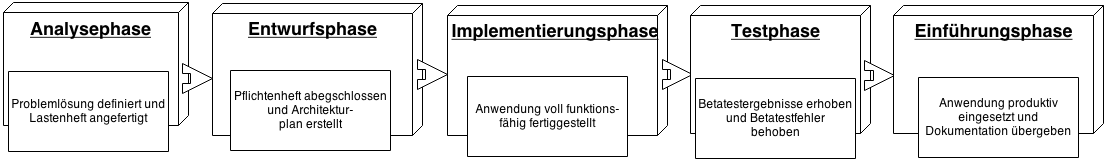
\includegraphics[width=1.0\textwidth]{Phasenplan.png}
\caption[Phasenplan des Projektes]{Phasenplan des Projektes\protect\footnotemark}
\label{fig:MockupFrontend}
\end{figure}
\footnotetext{eigene Darstellung}

\begin{description}

  \item[Die Analysephase] ist Ausgangspunkt der vorliegenden Projektarbeit. Sie setzt
  auf der aktuellen Ist-Situation an und in ihr werden Lösungsmöglichkeiten für
  das vorhandene Problem analysiert. Am Ende der Analysephase steht eine
  konzeptionelle Problemlösung. Das bedeutet konkret, aus der Analyse der
  vorliegenden Situation werden verschiedene Lösungsansätze entwickelt. Im
  Zuge der Analyse und Auswertung dieser Lösungsansätze wird ein Ansatz
  ausgewählt, der für die Lösung am geeignetsten ist. Die Analysephase ist in
  der vorliegenden Ausarbeitung im \verweis{Konzeptionierung} beschrieben.

  Die Ergebnisse der Analyse werden in einem Lastenheft\footnote{\citet{lastenheft2013}} formuliert.

  Die Analysephase wird mit dem Meilenstein "`Problemlösung definieren und
  Lastenheft angefertigt"' abgeschlossen.

  \item[Die Entwurfsphase] folgt im Anschluss auf die Analysephase.
  Ausgangspunkt der Entwurfsphase ist ein angefertigtes Lastenheft. Aufgrund der
  darin beschriebenen Anforderungen kann die Planung der Umsetzung
  begonnen werden. Die
  Entwurfsphase beinhaltet dabei Modelle und Entwürfe, 
  die konkret beschreiben, wie die
  Anforderungen des Lastenheftes umgesetzt werden. Das Ergebnis der Entwurfsphase ist ein erstelltes Pflichtenheft, das die konkretisierte Umsetzung des Problems
  beschreibt.

  Im vorliegenden Projekt wurden systematisch verschiedene Teilgebiete der
  entstehenden Lösung betrachtet und mit Modellen individuell konzipiert, um die
  Komplexität einer solchen Lösung in kleinere Teilbereiche zu unterteilen. Dabei
  wurden hauptsächlich die Bereiche Datenhaltung bzw. Datenbankdesign und
  Anwendungslogik voneinander getrennt betrachtet. Dieser getrennten Betrachtung
  ging dabei der Entwurf eines ersten Oberflächendesigns, ein sogenanntes
  Mockup, voraus. Mit diesem Mockup konnte ein erster Eindruck über Umfang und
  Komplexität gewonnen und zusätzlich Funktionalität und Benutzung
  verdeutlicht werden. Eine Abbildung dieses Mockups ist an Anhang ~\ref{sec:Mockup} zu sehen.

  Eine genauere Betrachtung der Entwurfsphase würde an dieser Stelle zu weit führen,
  kann aber in \citet{modelierungUndBetrieb2014} nachgelesen werden.
  Das angefertigte Pflichtenheft kann in \citet{pflichtenheft2013} nachgelesen werden.

  Die Entwurfsphase wurde mit dem Meilenstein "`Pflichtenheft abgeschlossen und
  Architekturplan erstellt"' abgeschlossen.

  \item[Die Implementierungsphase] folgt im Anschluss an die Entwurfsphase und
  baut auf einem abgeschlossenen Pflichtenheft auf. Diese Phase ist sowohl die
  zeitlich größte Phase als auch die Entscheidende, da in dieser Phase alle im
  Vorfeld geplanten Schritte und Modelle umgesetzt werden. In der Phase der
  Implementierung werden, aufbauend auf den vorher angefertigten Entwürfen, die
  theoretischen Modelle in ausführbaren Quellcode umgesetzt. In dieser Phase
  zeigt sich vor allem die Qualität der angefertigten Modelle, denn am
  schnellsten lässt sich Software entwickeln, wenn das dazugehörige Modell
  1:1 in Quellcode übertragen werden kann. Allerdings ist das, aufgrund der
  Schwierigkeit eine Software in seiner Komplexität in einem Modell zu erfassen,
  häufig schwer zu erreichen. Bei unerwartetem Abweichen vom Modell muss daher
  die Konzeption der Software erneut überdacht werden, um eventuellen logischen
  Fehlern vorzubeugen. Der Prozess dieser Implementierung kann in der
  Ausarbeitung Modellierung und Betrieb in Kapitel 5. (Umsetzung) nachgelesen werden.

  Die Implementierungsphase endet mit dem Meilenstein "`Anwendung voll
  funktionsfähig fertiggestellt"'.

  \item[Die Testphase] baut auf der fertigestellten und funktionierenden Software auf.
  Idealerweise wird der Test der Software von Personen durchgeführt, die nicht im Prozess der
  Softwareentwicklung beteiligt waren. Diese Personen haben eine
  unbeeinflusste Sicht auf die Software. Sie können so zum einen dessen
  intuitive Bedienung besser einschätzen und zum anderen benutzen sie die Software auch
  unvoreingenommen.Dies kann dazu führen, das sie Fehler in der Bedienung oder
  im Programm entdecken.Einen solchen Test, der von außenstehenden Personen
  durchgeführt wird, wird als Betatest bezeichnet. Diesem Betatest ist im
  Idealfall ein Alphatest der Entwickler vorausgegangen, in dem sie die entwickelten Anwendungsfälle (use cases) im fertigen Programm simulieren und dabei mögliche
  Fehler entdecken und ausbessern können. Der Alphatest wird in dieser Ausarbeitung nicht näher betrachtet,
  kann aber in \citet{modelierungUndBetrieb2014} nachgelesen werden.
  In der Betatestphase ist es besonders wichtig die  aufgetretenen Fehler
  und Kritiken zu erfassen und an die Entwickler weiterzugeben. Durch den
  Betatest können sogenannte "`Kinderkrankheiten"' früh erkannt und beseitigt
  werden. Das steigert die Qualität und erhöht vor allem die
  Benutzerzufriedenheit beim verwenden der Software. Die Betatestphase wird zudem im Folgenden
  zur Verifizierung von Projektzielen verwendet.\footnote{siehe \verweis{Zielkatalog}}

  Die Testphase wird mit dem Meilenstein "`Betatestergebnisse erhoben und
  Betatestfehler behoben"' abgeschlossen.

  \item[Die Einführungsphase] erfolgt nach erfolgreicher Fertigstellung der Software und Korrektur aller
  aufgetretenen Fehler. Die Software wird in dieser Phase dem Auftraggeber übergeben und produktiv eingesetzt.
  Zur Übergabe der Software gehört zudem eine Dokumentation der Funktionsweise, die im \verweis{Anwenderdokumentation} vorgestellt wird. Der Abschluss dieser Phase stellt damit den Abschluss des Projektes dar.

  Die Einführungsphase endet mit dem letzten Meilenstein "`Anwendung produktiv
  eingesetzt und Dokumentation übergeben"'.

\end{description}
\subsection{Projektrealisierung}
\label{sec:Projektrealisierung}

Aufbauend auf der Festlegung der Projektphasen kann das Projekt iterativ anhand der aufgezeigten Organisation
realisiert werden. An dieser Stelle setzt die konkrete Beschreibung der Realiesierung des
Projektes in \citet{modelierungUndBetrieb2014} an.
Ein Einblick in diese Realesierung wäre an dieser Stelle zu umfassend und zu komplex. Aus diesem Grund werden an dieser
Stelle nur die Ergebnisse der Projektrealsierung vorgestellt.

Realisiert werden sollte eine visuelle Ansicht des neuen Campus Lingen, in dem sich der Benutzer im Stile von Google
Street View frei umsehen kann. Diese Realiserung ist gelungen und das Eregbnis ist in \abbildung{FrontendFinal}
zu sehen:

\clearpage

\begin{figure}[htb] 
\centering
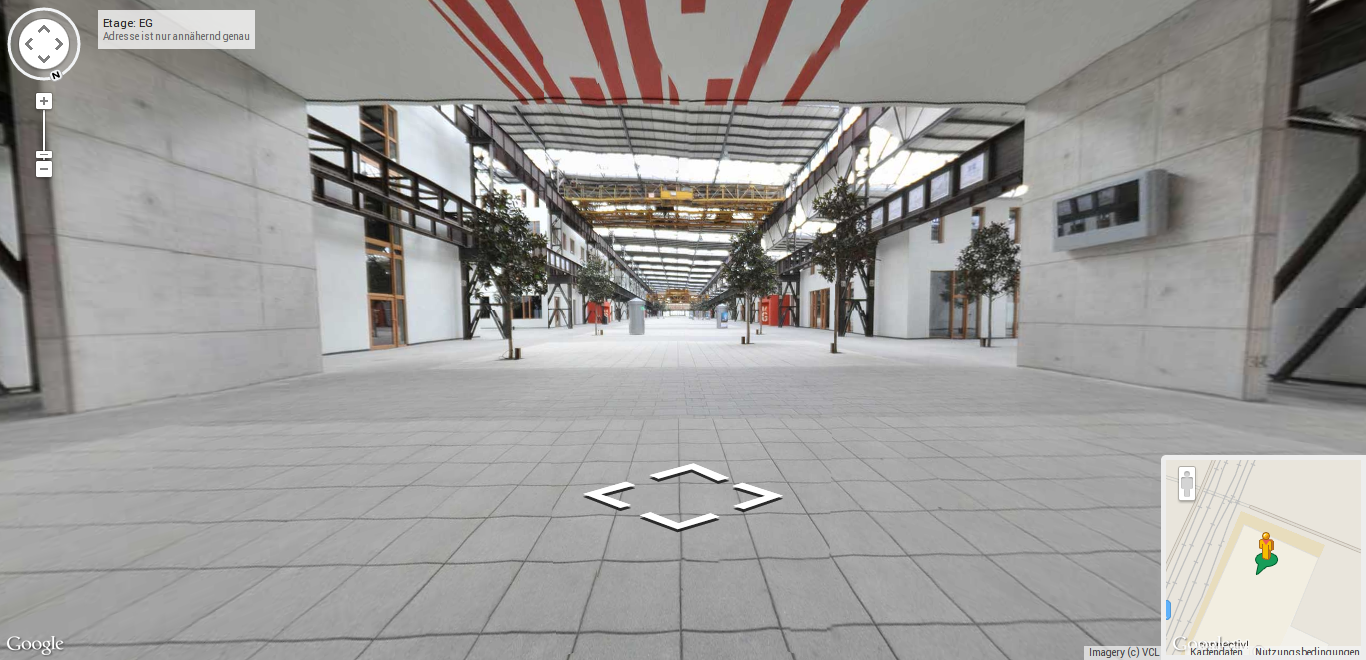
\includegraphics[width=1.0\textwidth]{FrontendFinal.png}
\caption[Abbildung der Benutzeransicht]{Ein Bildschirmfoto der fertigen Benutzeransicht\protect}
\label{fig:FrontendFinal}
\end{figure}

Neben dieser Benutzeransicht sollte darüber hinaus vor allem die Nachhaltigkeit des Projektes gewahrt werden.
Hierzu sollte ein Administrationsbereich entwickelt werden, in dem es möglich ist alle Informationen
der Benutzeransicht zu pflegen. Ein Ausschnit dieses Administrationsbereiches ist 
in \abbildung{BackendFinal} dargestellt:

\begin{figure}[htb] 
\centering
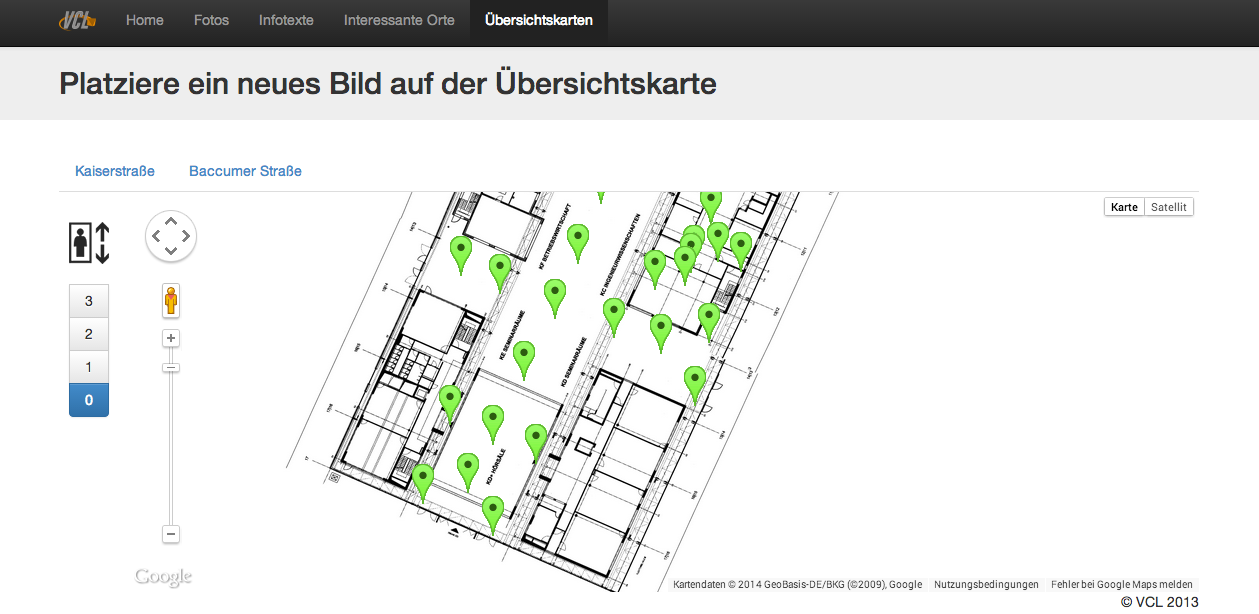
\includegraphics[width=1.0\textwidth]{BackendFinal.png}
\caption[Ausschnitt des Administrationsbereiches]{Verwalten und Platzieren von Panoramafotos im Administrationsbereich\protect}
\label{fig:BackendFinal}
\end{figure}
\subsection{Betrachtung der IT-Sicherheit}
\label{sec:BetrachtungDerItSicherheit}

% TODO: Wirklich schreiben???
SQLi und HTTPs durch Zertifikate.
\subsection{Projekttest}
\label{sec:Projekttest}

Der Projekttest dient im vorliegenden Projekt zur Verifikation der beschriebenen
Projektziele und zur Behebung von Fehlern innerhalb der Anwendung. Der
Projekttest gliedert sich dabei in zwei aufeinander folgende Phasen. In der
ersten Phase wird das Projekt vom Entwicklerteam selbst, anhand von erstellten
Anwendungsfällen, getestet. Einen solchen Test bezeichnet man als Alphatest, da
dieser von Personen durchgeführt wird, die an der Entwicklung beteiligt waren.
Der Alphatest dient primär zur Erkennung und Beseitigung von Fehlern in der
Anwendung. Der Abschluss dieses Test verifiziert, dass die Anwendung fehlerfrei
funktioniert. Aufbauend auf dem Alphatest wird ein Betatest der Anwendung von
aussenstehenden Personen durchgeführt. Dieser Test dient primär zur
Verifizierung der Projektziele. Der Alphatest wird an dieser Stelle nicht weiter
vertieft, da dieser für die Betrachtung des vorliegenden Themenbereiches nicht
relevant ist. Die Durchführung und Ergbnisse können in
\citet{modelierungUndBetrieb2014} im Kapitel 6 (Test) nachgelesen werden. Der
Fokus des Projekttests liegt im Folgenden auf dem durchgeführten Betatest.

Zur Durchführung des Betatests wurde im ersten Schritt ein definierter Bereich
des Campus in die erstellte Anwendung eingepflegt. Dieser Bereich zeigt den
Betatestern einen repräsentativen Ausschnitt des Campus.
Im zweiten Schritt wurde ein Onlinefragebogen vorbereitet, der von Betatestern
nach Benutzung der Anwendung ausgefüllt werden soll. Dieser Fragebogen enthält 
sowohl Fragen, die der Verifizierung der Zielerreichung dienen, als auch
Fragen, die dem Entwicklerteam Auskunft über mögliche Schwachstellen des Systems geben.
Da an dieser Stelle nur der Teil der Fragen, der zur Verifikation der Ziele dient,
interessant ist, wird nur ein Auschnitt des gesamten Fragebogens in\tabelle{Fragebogen} dargestellt.

An dem Betatest haben insgesamt 97 Personen teilgenommen. Die Auswertung der Tests ist in nachfolgender Tabelle
festgehalten:

\clearpage
\tabelleEinfg{Auswertung des Betatests}{tab:Fragebogen}{AuswertungBetatest}

Aufbauend auf diesen Ergebnissen erfolgt die Verifikation der Zielerreichung in \verweis{Zielerreichung}.
Der subjektive Eindruck der Betatester, der in obiger Tabelle in der letzten Spalte abzulesen ist,
zeigt dem Entwicklerteam aber bereits eine erste positive Resonanz.
\subsection{Anwenderdokumentation}
\label{sec:Anwenderdokumentation}

Zur Gewährleistung der Nachhaltigkeit ist es Ziel des Projektes eine
Dokumentation zu erstellen, die die Administrations- und Pflegefunktionen der
Anwendung erläutern. Der grobe Inhalt dieser Dokumentation wird im Folgenden
kurz vorgestellt, um einen Überblick über die Pflege der Anwendung zu geben. Die
vollständige Version kann in \citet{projektdokumentation2014} nachglesen werden.

Die Dokumentation umfasst die folgenden Teilbereiche:

\begin{itemize}
  \item Hinzufügen und Ändern von Fotos
  \item Hinzufügen und Ändern von Infotexten
  \item Hinzufügen und Ändern von interessanten Orten
  \item Positionieren von Fotos
  \item Zuordnung von Infotexten und Fotos
  \item Festlegen von Nachbarschaftsbeziehungen zwischen Fotos
\end{itemize}

Bei Pflege der Anwendung müssen in erster Linie Fotos, Infotexte und interessante Orte gepflegt werden. Die \textbf{Fotos}
sind dabei das Basiselement der Anwendung. Hier müssen Panoramabilder angefertigt und in kleinere Bildteile zerschnitten
werden. Die Hintergründe zu dieser Vorgehensweise werden in \citet{modelierungUndBetrieb2014} im
Kapitel 5.1 (Panoramaerstellung) beschrieben.
Die \textbf{Infotexte} dienen zum Anzeigen von relevanten Informationen auf einem Foto. In Infotexten können
zum Beispiel Projekte vorgestellt oder Öffnungszeiten von Gebäuden angezeigt werden. Die gesamte Informationsvermittlung
findet im Projekt über Infotexte statt.
Zum Navigieren durch den Campus stehen dem Benutzer zum einen die Navigationspfeile und zum anderen die
\textbf{interessanten Orte} zur Verfügung. Dem Benutzer wird durch Klick auf die
Übersichtskarte eine Liste mit Orten angezeigt, zu denen er springen kann.
Diese Navigationsmöglichkeit hilft Studieninteressierten schnell Orte, wie die
Bibliothek oder das Fachbereichsgebäude zu finden, ohne dass sie diese suchen
müssen. Diese interessanten Orte müssen aber im Administrationsbereich der
Anwendung hinterlegt und gepflegt werden.

Aufbauend auf der Pflege dieser Grundinformationen müssen in der Anwendung noch
weiterführende Zusatzinformationen gepflegt werden. Dazu zählt zum einem das
Positionieren des Fotos auf einer topographischen Karte, die Zuordnung zu
Infotexten und das Festlegen von Nachbarschaftsbeziehungen. Ist ein Foto
positioniert, kann es dem Benutzer im Frontend angezeigt werden. 
Sollen auf diesem Foto zusäzlich ein oder mehrere Infotexte angezeigt werden,
müssen die entsprechende Infotexte an das Foto angehängt werden. Diese Zuordnung
wird im Administrationsbereich gepflegt. Ebenso wird die angesprochene
Navigation zwischen zwei Fotos über die Navigationspfeile im
Administrationsbereich gepflegt. Dazu müssen zu jedem hochgeladenen und
positionierten Foto Nachbarfotos definiert werden. Diese Nachbarfotos werden dem
Benutzer als Navigationspfeile angezeigt.

\subsection{Projektabschluss}
\label{sec:Projektabschluss}

Das Projekt Virtueller Campus Lingen ist mit abschließender Fertigstellung der Anwenderdokumentation
abgeschlossen. Das Projekt muss in dieser Projektphase dem Auftraggeber übergeben werden.
Das zu übergebende Projekt besteht dabei aus den folgenden Teilen:

\begin{itemize}
  \item den vollständigen Quellcode der Software
  \item eine Kopie der Datenbank nach Abschluss des Projektes (Sicherheitskopie)
  \item die Installation der Webanwendung auf einem Webserver
  \item die Internetadresse der Anwendung und alle benötigten Passwörter
  \item eine Einführung in die Verwendung der Software anhand der Dokumentation
\end{itemize}

Auf Basis dieser Informationen und Materialien ist der Auftraggeber in der Lage das Projekt zu pflegen und zu erweitern. Die Wahrung der Nachhaltigkeit ist damit vollständig gewährleistet. Die Installation und Übergabe der Webanwendung ist für Mitte Juli 2014 geplant.